\documentclass[a4paper,twoside]{book}

\usepackage{graphicx}
\usepackage[pdftex]{hyperref}
\usepackage{fancyvrb}

\usepackage{makeidx}
\makeindex

\hypersetup{a4paper=true,
            plainpages=false,
            colorlinks=true,
            pdfpagemode=UseOutlines,	% FullScreen, UseNone, UseOutlines, UseThumbs
            bookmarksopen=true,
            bookmarksopenlevel=2,
            colorlinks=true,
            linkcolor=blue,
            urlcolor=blue,
            breaklinks=true,
            pdfstartview=FitH,		% Fit, FitH, FitV, FitBH
            pagebackref=true,
            pdfhighlight=/I,
            baseurl={http://www.rizauddin.com/},
            pdftitle={Document processing with LyX and SGML},
            pdfsubject={LaTeX},
            pdfauthor={Copyright \textcopyright 2004-2018, Rizauddin Saian},
            pdfkeywords={LaTeX}
}

\newenvironment{dedication}
{
    \cleardoublepage
    \thispagestyle{empty}
    \vspace*{\stretch{1}}
    \hfill\begin{minipage}[t]{0.66\textwidth}
        \raggedright
    }%
    {
    \end{minipage}
    \vspace*{\stretch{3}}
    \clearpage
}

%%%%%%%%%%%%%

\title{A Simple \LaTeX\ Tutorial}
\author{Rizauddin Saian \\ 
    Faculty of Computer \& Mathematical Sciences \\
    Universiti Teknologi MARA, Perlis}
%\date{July 11, 2018}

\renewcommand{\chaptername}{Tutorial}


\begin{document}
    
\maketitle

\pagenumbering{roman}

\frontmatter
% ... other frontmatter

\begin{dedication}
    To my wife and daughters.
\end{dedication}


\tableofcontents
\chapter{Preface}


\section*{How to Contact Us}
Please address comments and questions concerning this book to:\\
\begin{quote}
Rizauddin Saian\\
Faculty of Computer \& Mathematical Sciences \\
Universiti Teknologi MARA, Perlis\\
Email: rizauddin@uitm.edu.my
\end{quote}

\section*{Acknowledgements}
A big thank you to my family and all my students.

\listoffigures

\mainmatter 

\pagenumbering{arabic}

\chapter{Your First \LaTeX{} Document}
\label{chap:firstLaTeX}

\begin{figure}[h]
    \centering
    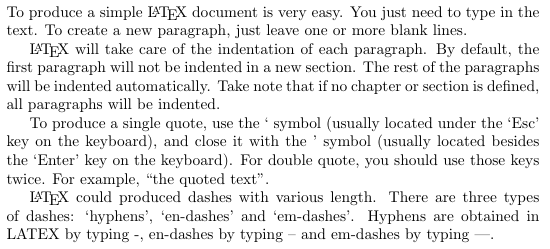
\includegraphics[width=0.7\linewidth]{img/tut1}
    \caption{Your first \LaTeX document.}
    \label{fig:tut1}
\end{figure}

\index{article} \index{a4paper} \index{12pt}
\begin{Verbatim}[frame=single]

\documentclass[a4paper,12pt]{article}
\begin{document}

To produce a simple \LaTeX{} document is very easy. You just
need to type in the text. To create a new paragraph,
just leave one or more blank lines.

\LaTeX{} will take care of the indentation of each paragraph.
By default, the first paragraph will not be indented in 
a new section. The rest of the paragraphs will be indented
automatically. Take note that if no chapter or section is 
defined, all paragraphs will be indented.

To produce a single quote, use the ` symbol (usually located
under the `Esc' key on the keyboard), and close it with 
the ' symbol (usually located besides the `Enter' key 
on the keyboard).
For double quote, you should use those keys twice. For
example, ``the quoted text''.

\LaTeX{} could produced dashes with various length. 
There are three types of dashes: `hyphens', `en-dashes'
and `em-dashes'. Hyphens are obtained in LATEX by 
typing -, en-dashes by typing -- and em-dashes by 
typing ---.

\end{document}

\end{Verbatim}

\noindent\textbf{Note:}

\begin{description}

	\item[en-dashes]\index{en-dash} to specify range of numbers, for example, ``on pages 12--20''
	\item[em-dashes]\index{em-dash} used for punctuating, for example, ``\LaTeX{} is a good text 
	processing software---trust me.''
\end{description}

\chapter{Title Page}
\label{chap:titlePage}
\begin{figure}[h]
    \centering
    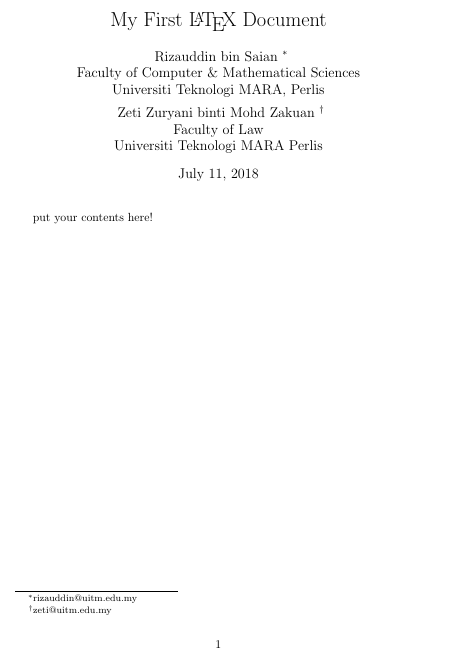
\includegraphics[width=0.75\linewidth]{img/tut2}
    \caption{The title page.}
    \label{fig:tut2}
\end{figure}

\index{title} \index{author} \index{article} \index{date} \index{today} \index{maketitle}
\begin{Verbatim}[frame=single]
\documentclass{article}

\title{My First \LaTeX{} Document}
\author{
Rizauddin bin Saian \thanks{rizauddin@uitm.edu.my} \\
Faculty of Computer \& Mathematical Sciences \\
Universiti Teknologi MARA, Perlis
\and
Zeti Zuryani binti Mohd Zakuan \thanks{zeti@uitm.edu.my} \\
Faculty of Law \\
Universiti Teknologi MARA Perlis
}

\date{\today}

\begin{document}
\maketitle

Put your contents here!

\end{Verbatim}


\chapter{List}
\label{chap:list}

\begin{figure}[h]
    \centering
    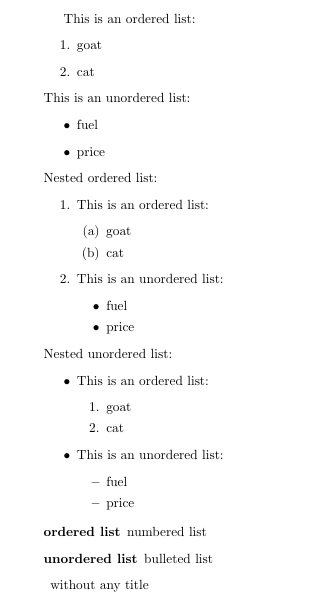
\includegraphics[width=0.6\linewidth]{img/tut3}
    \caption{List.}
    \label{fig:tut3}
\end{figure}



\index{enumerate} \index{item} \index{itemize}
\index{list}
\begin{Verbatim}[frame=single]

\documentclass{article}
\begin{document}

This is an ordered list:
\begin{enumerate}
\item goat
\item cat
\end{enumerate}

\noindent This is an unordered list:
\begin{itemize}
\item fuel
\item price
\end{itemize}

\noindent Nested ordered list:
\begin{enumerate}
	\item This is an ordered list:
	\begin{enumerate}
	\item goat
	\item cat
	\end{enumerate}
	
	\item This is an unordered list:
	\begin{itemize}
	\item fuel
	\item price
	\end{itemize}
\end{enumerate}

\noindent Nested unordered list:
\begin{itemize}
	\item This is an ordered list:
	\begin{enumerate}
	\item goat
	\item cat
	\end{enumerate}
	
	\item This is an unordered list:
	\begin{itemize}
	\item fuel
	\item price
	\end{itemize}
\end{itemize}

\begin{description}
	\item[ordered list] numbered list
	\item[unordered list] bulleted list
	\item without any title
\end{description}
\end{document}

\end{Verbatim}


\chapter{Table}
\label{chap:table}

\begin{figure}[h]
    \centering
    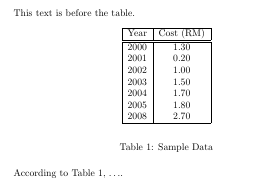
\includegraphics[width=0.7\linewidth]{img/tut4}
    \caption{Table.}
    \label{fig:tut4}
\end{figure}

\index{table} \index{center} \index{tabular}
\index{hline} \index{ref} \index{hline}
\begin{Verbatim}[frame=single]

\documentclass{article}

\begin{document}
This text is before the table.

\begin{table}[h]
	\begin{center}
		\begin{tabular}{|c|c|} \hline
			Year & Cost (RM)  \\
			\hline \hline
			2000 & 1.30 \\
			2001 & 0.20  \\
			2002 & 1.00  \\
			2003 & 1.50  \\
			2004 & 1.70  \\
			2005 & 1.80  \\
			2008 & 2.70  \\
			\hline
		\end{tabular}
	\end{center}
\caption {Sample Data}
\label{tab:TheCost}
\end{table}

According to Table~{\ref{tab:TheCost}}, $\dots$.

\end{document}

\end{Verbatim}

\section{Spanning the table}
\label{sec:spanningTheTable}

\begin{figure}[h]
    \centering
    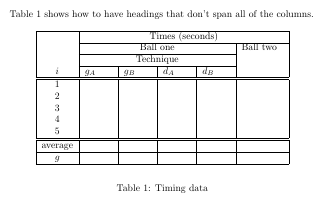
\includegraphics[width=0.7\linewidth]{img/tut4-1}
    \caption{Spanning the table.}
    \label{fig:tut4}
\end{figure}

\index{multicolumn} \index{tabular} \index{table} \index{center} \index{tabular} \index{label} \index{caption} \index{hline} \index{cline}
\begin{Verbatim}[frame=single]
\documentclass{article}

\begin{document}
Table~{\ref{tab:ngdata}} shows how to have headings
that don't span all of the columns.
\begin{table}[ht!]
\begin{center}
\begin{tabular}{|c|p{1cm}|p{1cm}|p{1cm}|p{1cm}|p{1.5cm}|} \hline
&\multicolumn{5}{|c|}{Times (seconds)} \\ \cline{2-6}
&\multicolumn{4}{|c|}{Ball one}& Ball two \\ \cline{2-5}
&\multicolumn{4}{|c|}{Technique} &\\ \cline{2-5}
$i$ & $g_A$  & $g_B$ & $d_A$ & $d_B$ & \\ \hline \hline
1 & & & & &   \\
2 & & & & &   \\
3 & & & & &   \\
4 & & & & &   \\
5 & & & & &   \\
\hline \hline

average& & & & &  \\
\hline
$g$ & & & & &  \\
\hline
\end{tabular}
\end{center}
\caption {Timing data}
\label{tab:ngdata}
\end{table}

\end{document}
\end{Verbatim}

\section{The Table of Tables}
\label{sec:theTableOfTables}

\begin{figure}[h]
    \centering
    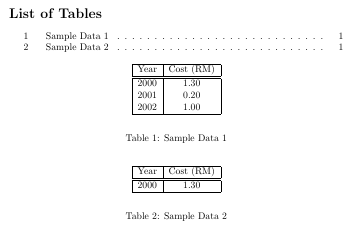
\includegraphics[width=0.7\linewidth]{img/tut4-2}
    \caption{The table of tables.}
    \label{fig:tut4-2}
\end{figure}

\index{listoftables} \index{table} \index{center} \index{tabular} \index{label} \index{caption} \index{hline}
\begin{Verbatim}[frame=single]
\documentclass{article}

\begin{document}

\listoftables

\begin{table}[h]
\begin{center}
\begin{tabular}{|c|c|} \hline
Year & Cost (RM)  \\
\hline \hline
2000 & 1.30 \\
2001 & 0.20  \\
2002 & 1.00  \\
\hline
\end{tabular}
\end{center}
\caption {Sample Data 1}
\label{tab:TheCost}
\end{table}


\begin{table}[h]
\begin{center}
\begin{tabular}{|c|c|} \hline
Year & Cost (RM)  \\
\hline \hline
2000 & 1.30 \\
\hline
\end{tabular}
\end{center}
\caption {Sample Data 2}
\label{tab:TheCost}
\end{table}

\end{document}
\end{Verbatim}

\chapter{Figures}
\label{chap:figures}

\begin{figure}[h]
    \centering
    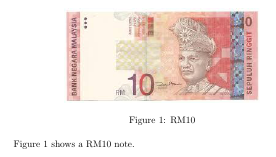
\includegraphics[width=0.7\linewidth]{img/tut5}
    \caption{Figures.}
    \label{fig:tut5}
\end{figure}

\index{graphicx} \index{includegraphics} \index{textwidth} \index{caption} \index{label} \index{figure} \index{centering}
\begin{Verbatim}[frame=single]
\documentclass{article}

\usepackage{graphicx}

\begin{document}
\begin{figure}[htbp]
\centering
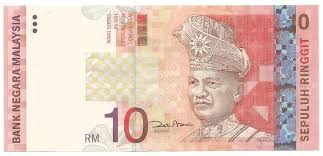
\includegraphics[width=0.6\textwidth]{ten}
\caption{RM10}
\label{fig:car}
\end{figure}

Figure~{\ref{fig:car}} shows a RM10 note.

\end{document}
\end{Verbatim}

\noindent You can also scale the picture using [scale=0.8]
instead of [width=0.6\textbackslash textwidth]

\section{Table of Figures}
\label{sec:tableOfFigures}

\begin{figure}[h]
\centering
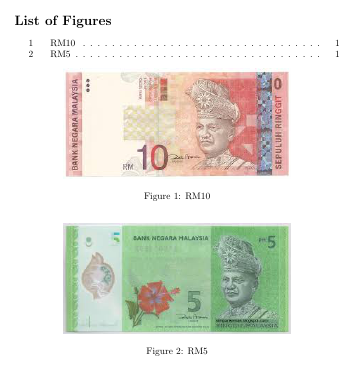
\includegraphics[width=0.7\linewidth]{img/tut5-1}
\caption{Table of figures.}
\label{fig:tut5-1}
\end{figure}


\begin{Verbatim}[frame=single]
\documentclass{article}
\usepackage{graphicx}

\begin{document}

\listoffigures

\begin{figure}[h]
\centering
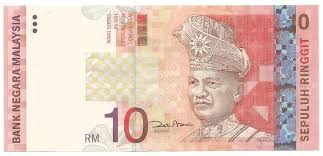
\includegraphics[width=0.7\linewidth]{ten}
\caption{RM10}
\label{fig:ten}
\end{figure}

\begin{figure}[h]
\centering
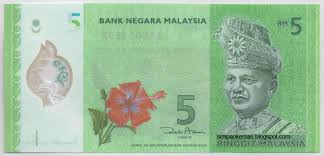
\includegraphics[width=0.7\linewidth]{five}
\caption{RM5}
\label{fig:five}
\end{figure}

\end{document}
\end{Verbatim}

\chapter{Document Styles}
\label{chap:documentStyles}

\section{Article document style}
\label{sec:articleDocumentStyle}

\begin{figure}[h]
    \centering
    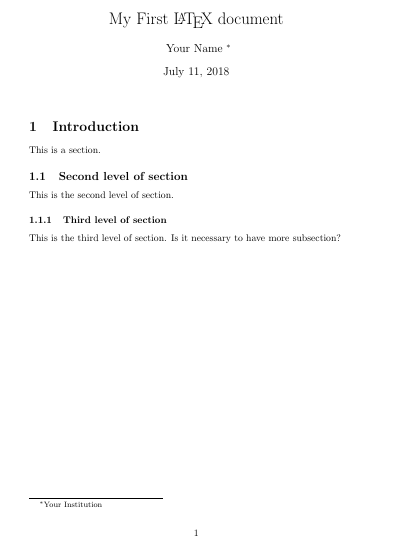
\includegraphics[width=0.7\linewidth]{img/tut6-1}
    \caption{Article document style.}
    \label{fig:tut6-1}
\end{figure}

\index{article} \index{section} \index{subsection}
\begin{Verbatim}[frame=single]
\documentclass{article}

\title{My First \LaTeX{} document}
\author{Your Name \thanks{Your Institution}}
\date{\today}

\begin{document}
\maketitle

\section{Introduction}

This is a section.

\subsection{Second level of section}

This is the second level of section.

\subsubsection{Third level of section}

This is the third level of section.
Is it necessary to have more subsection?

\end{document}
\end{Verbatim}

\section{Report document style}
\label{reportDocumentStyle}

\begin{figure}[ht!]
    \centering
    \begin{tabular}{c|c}
        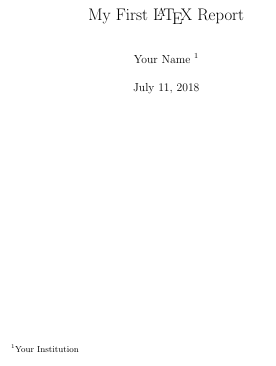
\includegraphics[width=0.3\linewidth]{img/tut6-2a} & 
        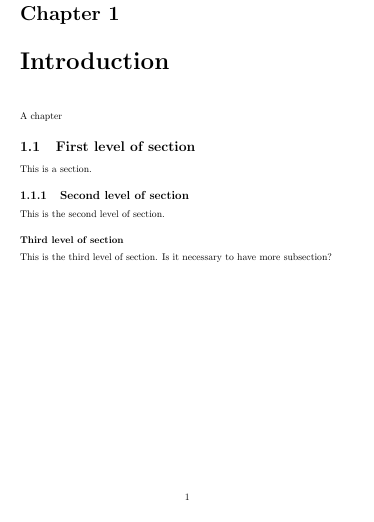
\includegraphics[width=0.3\linewidth]{img/tut6-2b} \\
    \end{tabular} 
    \caption{Report document style.}
    \label{fig:tut6-3a}
\end{figure}

\index{report} \index{chapter} \index{section} \index{subsection}
\begin{Verbatim}[frame=single]
\documentclass{report}

\title{My First \LaTeX{} Report}
\author{Your Name \thanks{Your Institution}}
\date{\today}

\begin{document}
\maketitle

\chapter{Introduction}

A chapter

\section{First level of section}

This is a section.

\subsection{Second level of section}

This is the second level of section.

\subsubsection{Third level of section}

This is the third level of section.
Is it necessary to have more subsection?

\end{document}
\end{Verbatim}

\section{Book document style}
\label{sec:bookDocumentStyle}

\begin{figure}[ht!]
    \centering
    \begin{tabular}{c|c}
        
\includegraphics[width=0.3\linewidth]{img/tut6-3a} & 
        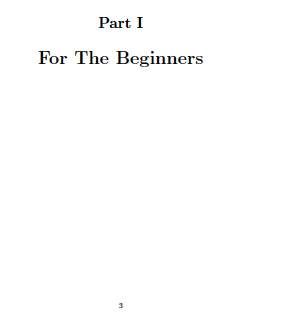
\includegraphics[width=0.3\linewidth]{img/tut6-3b} \\
        \hline \\
        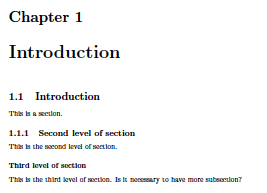
\includegraphics[width=0.3\linewidth]{img/tut6-3c}
    \end{tabular} 
    \caption{Book document style.}
    \label{fig:tut6-3a}
\end{figure}

\index{book} \index{part} \index{chapter} \index{section} \index{subsection} \index{subsubsection}
\begin{Verbatim}[frame=single]
\documentclass{book}

\title{My First \LaTeX{} Book}
\author{Your Name \thanks{Your Institution}}
\date{\today}

\begin{document}
\maketitle

\part{For The Beginners}

\chapter{Introduction}

\section{Introduction}

This is a section.

\subsection{Second level of section}

This is the second level of section.

\subsubsection{Third level of section}

This is the third level of section.
Is it necessary to have more subsection?

\end{document}

\end{Verbatim}

\chapter{Table of Contents}
\label{chap:tableOfContents}

To generate a table of contents, insert ``\textbackslash tableofcontents'' 
after the ``\textbackslash maketitle'' command.


\begin{figure}[h]
    \centering
    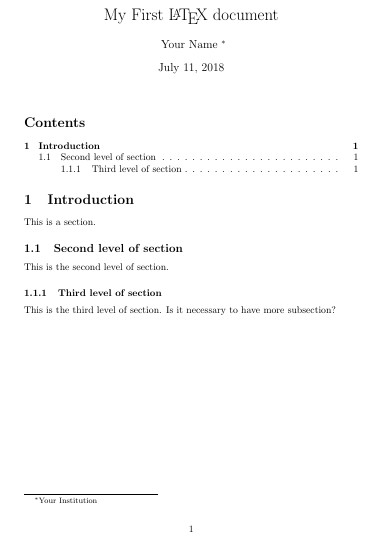
\includegraphics[width=0.7\linewidth]{img/tut7}
    \caption{The table of contents.}
    \label{fig:tut7}
\end{figure}

\index{tableofcontents}
\begin{Verbatim}[frame=single]

\documentclass{article}

\title{My First \LaTeX{} document}
\author{Your Name \thanks{Your Institution}}
\date{\today}

\begin{document}
\maketitle

\tableofcontents

\section{Introduction}

This is a section.

\subsection{Second level of section}

This is the second level of section.

\subsubsection{Third level of section}

This is the third level of section.
Is it necessary to have more subsection?

\end{document}
\end{Verbatim}

\chapter{Abstract}
\label{chap:abstract}

\begin{figure}[h]
    \centering
    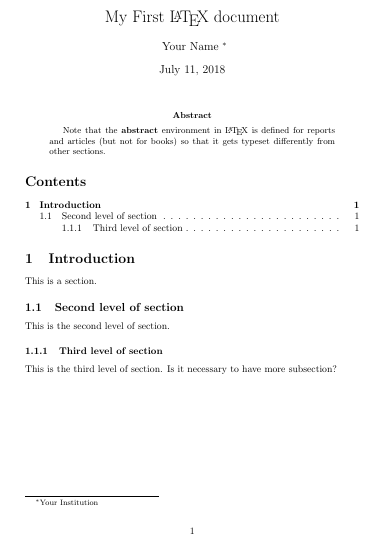
\includegraphics[width=0.75\linewidth]{img/tut8}
    \caption{The abstract.}
    \label{fig:tut8}
\end{figure}

\index{textbf} \index{abstract} \index{thanks} \index{today} \index{date}
\begin{Verbatim}[frame=single]

\documentclass{article}

\title{My First \LaTeX{} document}
\author{Your Name \thanks{Your Institution}}
\date{\today}

\begin{document}
\maketitle

\begin {abstract} 
Note that the \textbf{abstract} environment in \LaTeX\
is defined for 
reports and articles (but not for books) so 
that it gets typeset 
differently from other sections.
\end{abstract}

\tableofcontents

\section{Introduction}

This is a section.

\subsection{Second level of section}

This is the second level of section.

\subsubsection{Third level of section}

This is the third level of section.
Is it necessary to have more subsection?

\end{document}
\end{Verbatim}

\chapter{Bibliography}
\label{chap:bibliography}

\section{Plain format}
\label{sec:plainformat}

\begin{figure}[h]
    \centering
    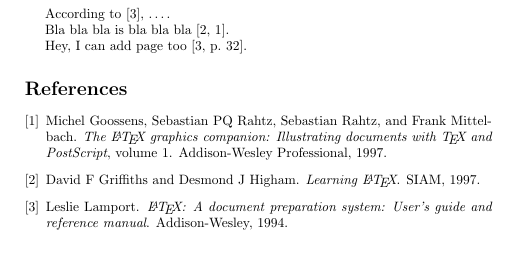
\includegraphics[width=0.7\linewidth]{img/tut9-1}
    \caption{Plain format.}
    \label{fig:tut9-1}
\end{figure}

\index{cite} \index{plain}
\begin{Verbatim}[frame=single]
\documentclass{article}

\begin{document}

According to \cite{lamport1994latex}, \dots.

Bla bla bla is bla bla bla \cite{griffiths1997learning, 
goossens1997latex}.

Hey, I can add page too \cite[p.~32]{lamport1994latex}.

\bibliographystyle{plain}
\bibliography{ref}

\end{document}
\end{Verbatim}

\begin{Verbatim}[frame=single]
%ref.bib
%random articles
@book{lamport1994latex,
title={{\LaTeX}: A document preparation system: User's guide 
and reference manual},
author={Lamport, Leslie},
year={1994},
publisher={Addison-Wesley}
}
@book{goossens1997latex,
title={The {\LaTeX} graphics companion: Illustrating documents 
with {\TeX} and PostScript},
author={Goossens, Michel and Rahtz, 
Sebastian PQ and Rahtz, Sebastian and Mittelbach, Frank},
volume={1},
year={1997},
publisher={Addison-Wesley Professional}
}
@book{griffiths1997learning,
title={Learning {\LaTeX}},
author={Griffiths, David F and Higham, Desmond J},
year={1997},
publisher={SIAM}
}
\end{Verbatim}


\section{APA Format}
\label{sec:APAformat}

\begin{figure}[h]
    \centering
    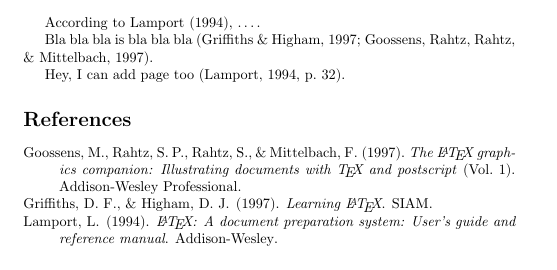
\includegraphics[width=0.7\linewidth]{img/tut9-2}
    \caption{APA format.}
    \label{fig:tut9-2}
\end{figure}

\index{citeA} \index{cite} \index{apacite}
\begin{Verbatim}[frame=single]
\documentclass{article}
\usepackage{apacite}

\begin{document}

According to \citeA{lamport1994latex}, \dots.

Bla bla bla is bla bla bla \cite{griffiths1997learning, 
goossens1997latex}.

Hey, I can add page too \cite[p.~32]{lamport1994latex}.

\bibliographystyle{apacite}
\bibliography{ref}

\end{document}
\end{Verbatim}

\section{IEEE Format}
\label{sec:IEEEformat}

\begin{figure}[h]
    \centering
    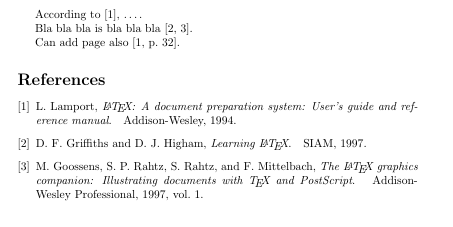
\includegraphics[width=0.7\linewidth]{img/tut9-3}
    \caption{IEEE Format.}
    \label{fig:tut9-3}
\end{figure}

\index{cite} \index{IEEEtranN} \index{natbib}
\begin{Verbatim}[frame=single]
\documentclass{article}

\usepackage[numbers]{natbib}
\begin{document}

According to \cite{lamport1994latex}, \dots.

Bla bla bla is bla bla bla
 \cite{griffiths1997learning, goossens1997latex}.

Can add page also \cite[p.~32]{lamport1994latex}.

\bibliographystyle{IEEEtranN}
\bibliography{ref}

\end{document}
\end{Verbatim}

%\clearpage
\cleardoublepage % for book class
\addcontentsline{toc}{chapter}{Index}
\printindex

\backmatter

\end{document}
